While a well-written DPC++ kernel without cross-work-item dependences can run in parallel effectively on a CPU, we can also apply vectorization to DPC++ kernels to leverage SIMD hardware, similarly to the GPU support described in Chapter 15. Essentially, CPU processors may optimize memory loads, stores, and operations using SIMD instructions by leveraging the fact that most data elements are often in contiguous memory and take the same control flow paths through a data-parallel kernel. For example, in a kernel with a statement a[i] = a[i] + b[i], each data element executes with same instruction stream load, load, add, and store by sharing hardware logic among multiple data elements and executing them as a group, which may be mapped naturally onto a hardware’s SIMD instruction set. Specifically, multiple data elements can be processed simultaneously by a single instruction.\par

The number of data elements that are processed simultaneously by a single instruction is sometimes referred to as the vector length (or SIMD width) of the instruction or processor executing it. In Figure 16-11, our instruction stream runs with four-way SIMD execution.\par

\hspace*{\fill} \par %插入空行
Figure 16-11. Instruction stream for SIMD execution
\begin{center}
	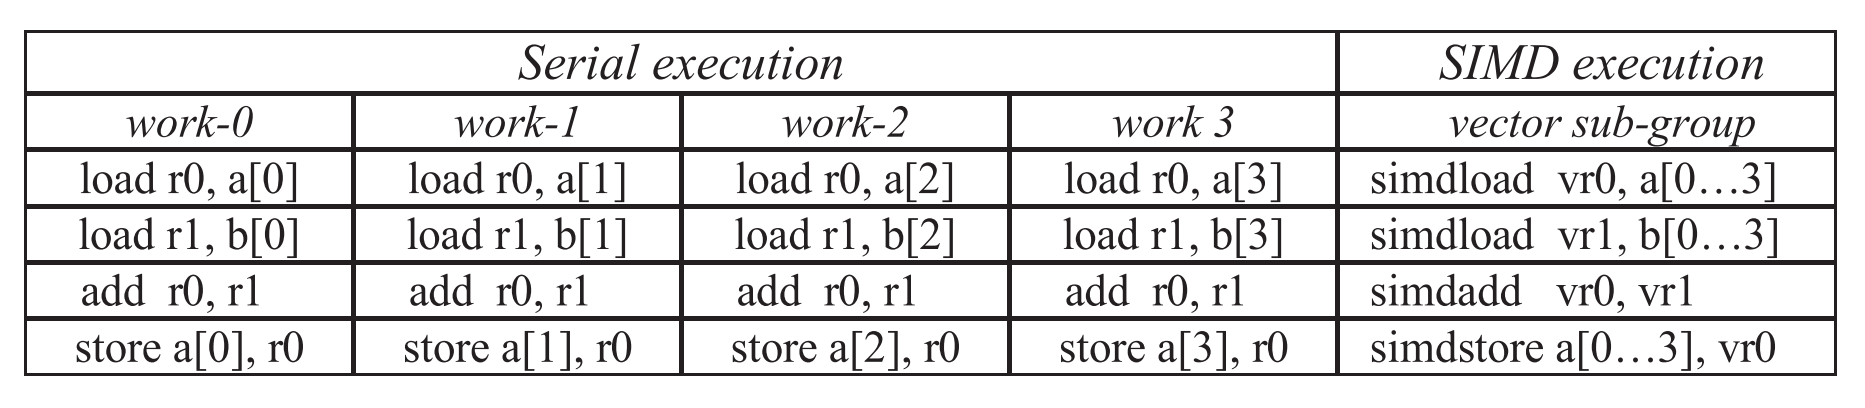
\includegraphics[width=1.0\textwidth]{content/chapter-16/images/10}
\end{center}

CPU processors are not the only processors that implement SIMD instruction sets. Other processors such as GPUs implement SIMD instructions to improve efficiency when processing large sets of data. A key difference with Intel Xeon CPU processors, compared with other processor types, is having three fixed-size SIMD register widths 128-bit XMM, 256-bit YMM, and 512-bit ZMM instead of a variable length of SIMD width. When we write DPC++ code with SIMD parallelism using sub-group or vector types, we need to be mindful of SIMD width and the number of SIMD vector registers in the hardware.\par

\hspace*{\fill} \par %插入空行
\textbf{Ensure SIMD Execution Legality}

Semantically, the DPC++ execution model ensures that SIMD execution can be applied to any kernel, and a set of work-items in each work-group (i.e., a sub-group) may be executed concurrently using SIMD instructions. Some implementations may instead choose to execute loops within a kernel using SIMD instructions, but this is possible if and only if all original data dependences are preserved, or data dependences are resolved by the compiler based on privatization and reduction semantics.\par

A single DPC++ kernel execution can be transformed from processing of a single work-item to a set of work-items using SIMD instructions within the work-group. Under the ND-range model, the fastest-growing (unit-stride) dimension is selected by the compiler vectorizer on which to generate SIMD code. Essentially, to enable vectorization given an NDrange, there should be no cross-work-item dependences between any two work-items in the same sub-group, or the compiler needs to preserve cross-work-item forward dependences in the same sub-group.\par

When the kernel execution of work-items is mapped to threads on CPUs, fine-grained synchronization is known to be costly, and the thread context switch overhead is high as well. It is therefore an important performance optimization to eliminate dependences between work-items within a work-group when writing a DPC++ kernel for CPUs. Another effective approach is to restrict such dependences to the work-items within a sub-group, as shown for the read-before-write dependence in Figure 16-12. If the sub-group is executed under a SIMD execution model, the sub-group barrier in the kernel can be treated by the compiler as a no-op, and no real synchronization cost is incurred at runtime.\par

\hspace*{\fill} \par %插入空行
Figure 16-12. Using a sub-group to vectorize a loop with a forward dependence
\begin{lstlisting}[caption={}]
using namespace sycl::intel;

queue Q;
range<2> G = {n, w};
range<2> L = {1, w};

int *a = malloc_shared<int>(n*(n+1), Q);

for (int i = 0; i < n; i++)
	for (int j = 0; j < n+1; j++) a[i*n + j] = i + j;
	
Q.parallel_for(nd_range<2>{G, L}, [=](nd_item<2> it)
	[[cl::intel_reqd_sub_group_size(w)]] {
		
	// distribute uniform "i" over the sub-group with 8-way
	// redundant computation
	const int i = it.get_global_id(0);
	sub_group sg = it.get_sub_group();
	
	for (int j = sg.get_local_id()[0]; j < n; j += w) {
		// load a[i*n+j+1:8] before updating a[i*n+j:8] to preserve
		// loop-carried forward dependence
		auto va = a[i*n + j + 1];
		sg.barrier();
		a[i*n + j] = va + i + 2;
	}
	sg.barrier();
	
}).wait();
\end{lstlisting}

The kernel is vectorized (with a vector length of 8), and its SIMD execution is shown in Figure 16-13. A work-group is formed with a group size of (1, 8), and the loop iterations inside the kernel are distributed over these sub-group work-items and executed with eight-way SIMD parallelism.\par

In this example, if the loop in the kernel dominates the performance, allowing SIMD vectorization across the sub-group will result in a significant performance improvement.\par

The use of SIMD instructions that process data elements in parallel is one way to let the performance of the kernel scale beyond the number of CPU cores and hyper-threads.\par

\hspace*{\fill} \par %插入空行
Figure 16-13. SIMD vectorization for a loop with a forward dependence
\begin{center}
	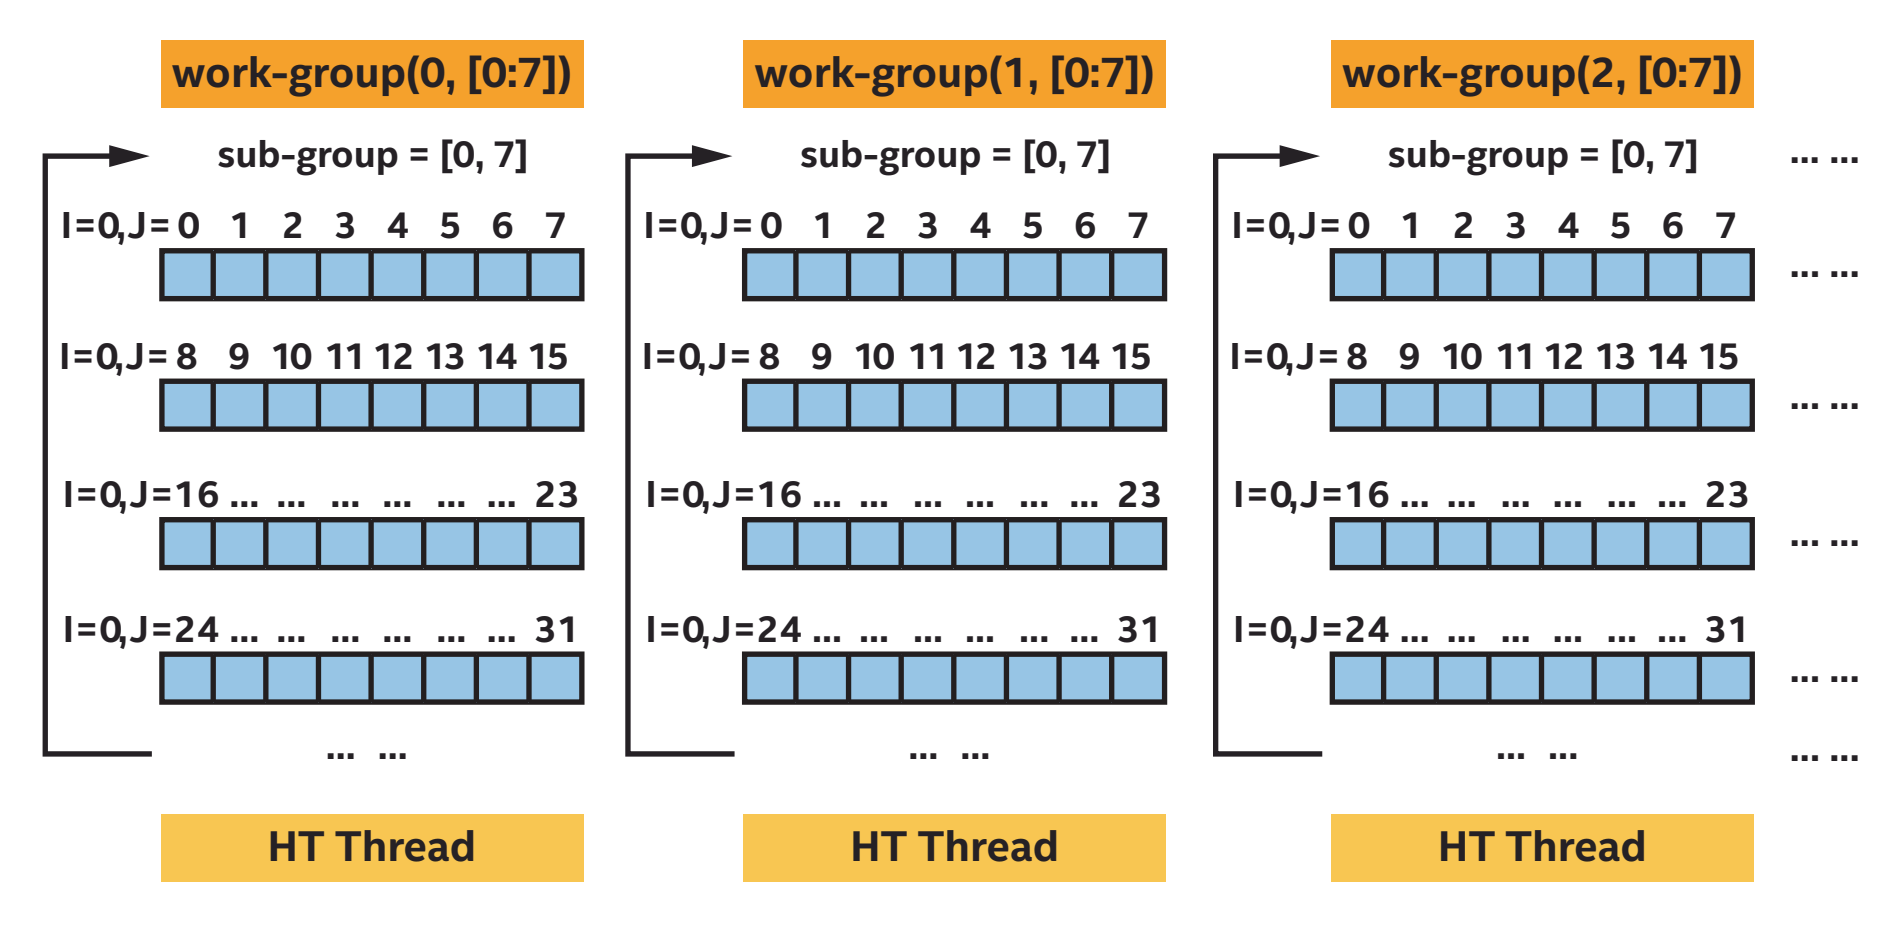
\includegraphics[width=1.0\textwidth]{content/chapter-16/images/7}
\end{center}

\hspace*{\fill} \par %插入空行
\textbf{SIMD Masking and Cost}

In real applications, we can expect conditional statements such as an if statement, conditional expressions such as a = b > a? a: b, loops with a variable number of iterations, switch statements, and so on. Anything that is conditional may lead to scalar control flows not executing the same code paths and, just like on a GPU (Chapter 15), can lead to decreased performance. A SIMD mask is a set of bits with the value 1 or 0, which is generated from conditional statements in a kernel. Consider an example with A={1, 2, 3, 4}, B={3, 7, 8, 1}, and the comparison expression a < b. The comparison returns a mask with four values {1, 1, 1, 0} that can be stored in a hardware mask register, to dictate which lanes of later SIMD instructions should execute the code that was guarded (enabled) by the comparison.\par

If a kernel contains conditional code, it is vectorized with masked instructions that are executed based on the mask bits associated with each data element (lane in the SIMD instruction). The mask bit for each data element is the corresponding bit in a mask register.\par

Using masking may result in lower performance than corresponding 
non-masked code. This may be caused by\par

\begin{itemize}
	\item An additional mask blend operation on each load
	\item Dependence on the destination
\end{itemize}

Masking has a cost, so use it only when necessary. When a kernel is an ND-range kernel with explicit groupings of work-items in the execution range, care should be taken when choosing an ND-range work-group size to maximize SIMD efficiency by minimizing masking cost. When a workgroup  size is not evenly divisible by a processor’s SIMD width, part of the work-group may execute with masking for the kernel.\par

\hspace*{\fill} \par %插入空行
Figure 16-14. Three masking code generations for masking in kernel
\begin{center}
	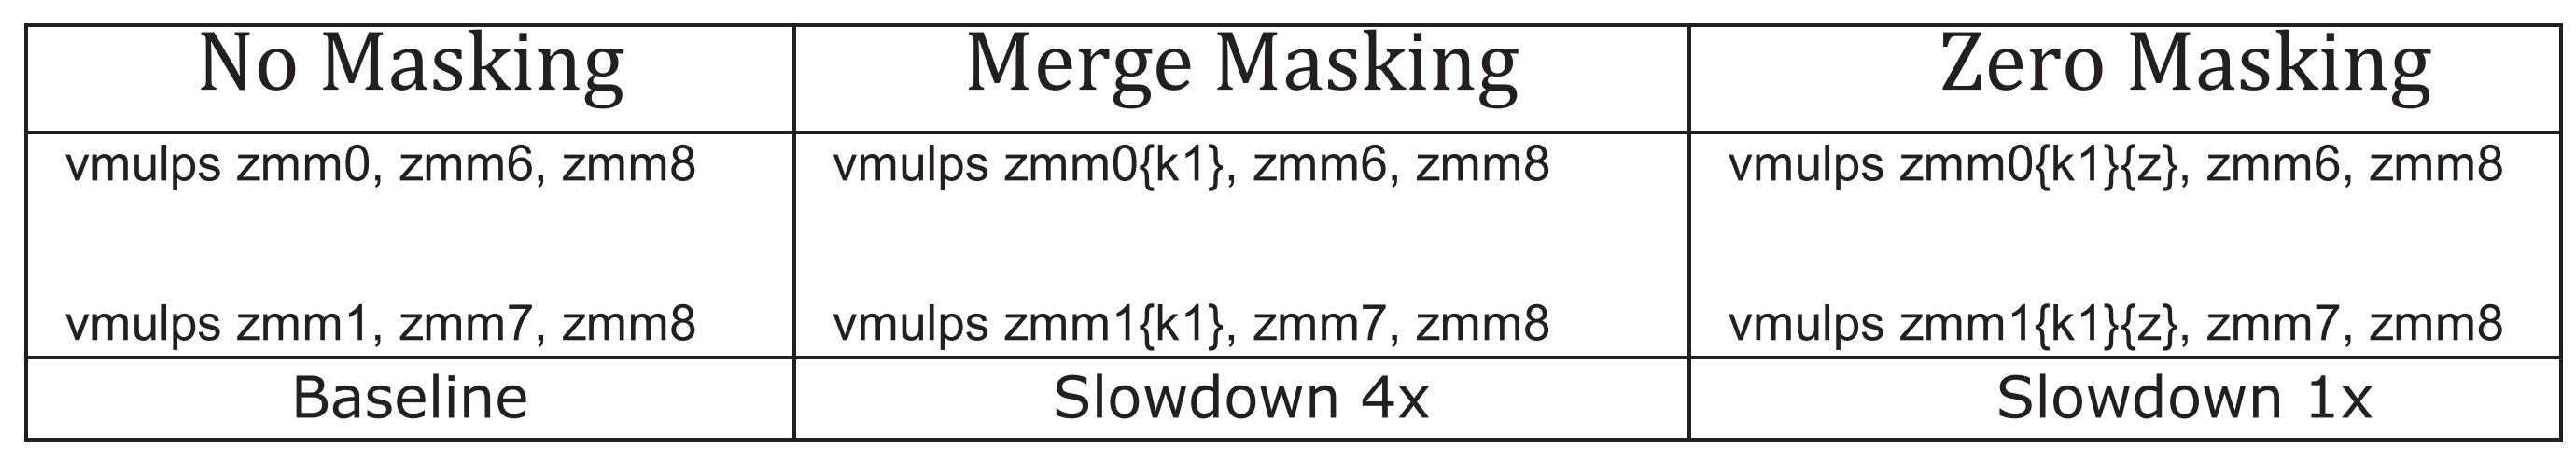
\includegraphics[width=1.0\textwidth]{content/chapter-16/images/11}
\end{center}

Figure 16-14 shows how using merge masking creates a dependence on the destination register:\par

\begin{itemize}
	\item With no masking, the processor executes two multiplies (vmulps) per cycle.
	\item With merge masking, the processor executes two multiplies every four cycles as the multiply instruction (vmulps) preserves results in the destination register as shown in Figure 16-17.
	\item Zero masking doesn’t have a dependence on the destination register and therefore can execute two multiplies (vmulps) per cycle.
\end{itemize}

Accessing cache-aligned data gives better performance than accessing non-aligned data. In many cases, the address is not known at compile time or is known and not aligned. In these cases, a peeling on memory accesses may be implemented, to process the first few elements using masked accesses, up to the first aligned address, and then to process unmasked accesses followed by a masked remainder, through multiversioning techniques in the parallel kernel. This method increases code size, but improves data processing overall.\par

\hspace*{\fill} \par %插入空行
\textbf{Avoid Array-of-Struct for SIMD Efficiency}

AOS (Array-of-Struct) structures lead to gathers and scatters, which can both impact SIMD efficiency and introduce extra bandwidth and latency for memory accesses. The presence of a hardware gather-scatter mechanism does not eliminate the need for this transformation—gatherscatter accesses commonly need significantly higher bandwidth and latency than contiguous loads. Given an AOS data layout of struct {float x; float y; float z; float w;} a[4], consider a kernel operating on it as shown in Figure 16-15.\par

\hspace*{\fill} \par %插入空行
Figure 16-15. SIMD gather in a kernel
\begin{lstlisting}[caption={}]
cgh.parallel_for<class aos<T>>(numOfItems,[=](id<1> wi) {
	x[wi] = a[wi].x; // lead to gather x0, x1, x2, x3
	y[wi] = a[wi].y; // lead to gather y0, y1, y2, y3
	z[wi] = a[wi].z; // lead to gather z0, z1, z2, z3 
	w[wi] = a[wi].w; // lead to gather w0, w1, w2, w3
});
\end{lstlisting}

When the compiler vectorizes the kernel along a set of work-items, it leads to SIMD gather instruction generation due to the need for non-unitstride memory accesses. For example, the stride of a[0].x, a[1].x, a[2].x and a[3].x is 4, not a more efficient unit-stride of 1.\par

\begin{center}
	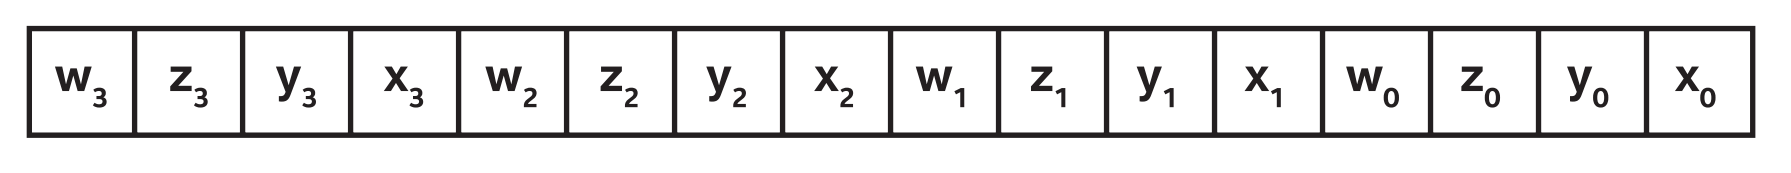
\includegraphics[width=1.0\textwidth]{content/chapter-16/images/8}
\end{center}

In a kernel, we can often achieve a higher SIMD efficiency by eliminating the use of memory gather-scatter operations. Some code benefits from a data layout change that converts data structures written in an Array-of-Struct (AOS) representation to a Structure of Arrays (SOA) representation, that is, having separate arrays for each structure field to keep memory accesses contiguous when SIMD vectorization is performed. For example, consider a SOA data layout of struct {float x[4]; float 	y[4]; float z[4]; float w[4];} a; as shown here:\par

\begin{center}
	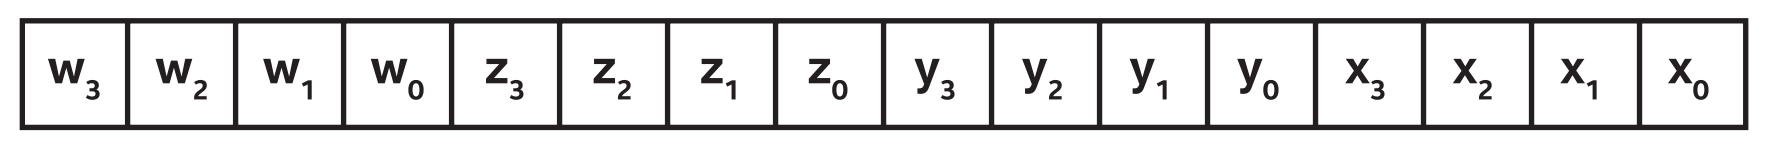
\includegraphics[width=1.0\textwidth]{content/chapter-16/images/9}
\end{center}

A kernel can operate on the data with unit-stride (contiguous) vector loads and stores as shown in Figure 16-16, even when vectorized!

\hspace*{\fill} \par %插入空行
Figure 16-16. SIMD unit-stride vector load in a kernel
\begin{lstlisting}[caption={}]
cgh.parallel_for<class aos<T>>(numOfItems,[=](id<1> wi) {
	x[wi] = a.x[wi]; // lead to unit-stride vector load x[0:4]
	y[wi] = a.y[wi]; // lead to unit-stride vector load y[0:4]
	z[wi] = a.z[wi]; // lead to unit-stride vector load z[0:4]
	w[wi] = a.w[wi]; // lead to unit-stride vector load w[0:4]
});
\end{lstlisting}

The SOA data layout helps prevent gathers when accessing one field of the structure across the array elements and helps the compiler to vectorize kernels over the contiguous array elements associated with work-items. Note that such AOS-to-SOA or AOSOA data layout transformations are expected to be done at the program level (by us) considering all the places where those data structures are used. Doing it at just a loop level will involve costly transformations between the formats before and after the loop. However, we may also rely on the compiler to perform vector-load-and-shuffle optimizations for AOS data layouts with some cost. When a member of SOA (or AOS) data layout has a vector type, the compiler vectorization will perform either horizontal expansion or vertical expansion as described in Chapter 11 based on underlying hardware to generate optimal code.\par

\hspace*{\fill} \par %插入空行
\textbf{Data Type Impact on SIMD Efficiency}

C++ programmers often use integer data types whenever they know that the data fits into a 32-bit signed type, often leading to code such as\par

\begin{tcolorbox}[colback=white,colframe=black]
int id = get\_global\_id(0); a[id] = b[id] + c[id];
\end{tcolorbox}

However, given that the return type of the get\_global\_id(0) is size\_t(unsigned integer, often 64-bit), in some cases, the conversion reduces the optimization that a compiler can legally perform. This can then lead to SIMD gather/scatter instructions when the compiler vectorizes the code in the kernel, for example

\begin{itemize}
	\item Read of a[get\_global\_id(0)] leads to a SIMD unitstride vector load.
	\item Read of a[(int)get\_global\_id(0)] leads to a nonunit-stride gather instruction.
\end{itemize}

This nuanced situation is introduced by the wraparound behavior (unspecified behavior and/or well-defined wraparound behavior in C++ standards) of data type conversion from size\_t to int (or uint), which is mostly a historical artifact from the evolution of C-based languages. Specifically, overflow across some conversions is undefined behavior, which actually allows the compiler to assume that such conditions never happen and to optimize more aggressively. Figure 16-17 shows some examples for those wanting to understand the details.\par

\hspace*{\fill} \par %插入空行
Figure 16-17. Examples of integer type value wraparound
\begin{center}
	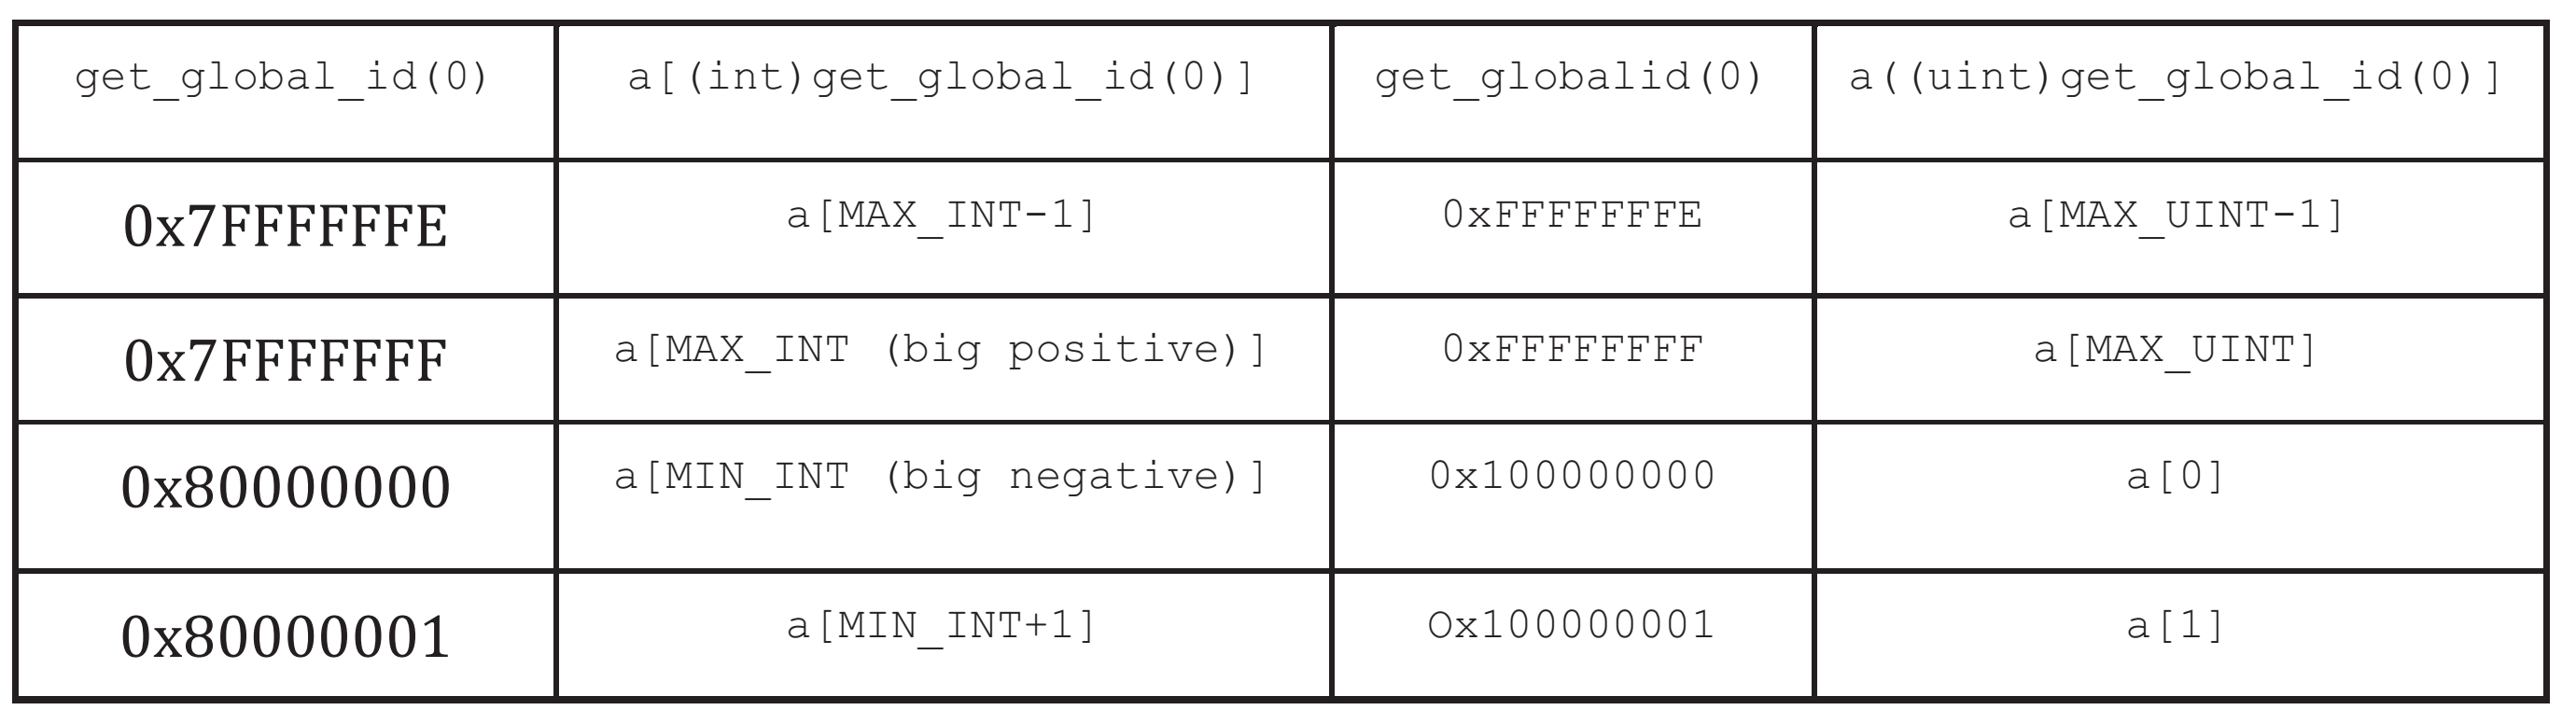
\includegraphics[width=1.0\textwidth]{content/chapter-16/images/12}
\end{center}

SIMD gather/scatter instructions are slower than SIMD unit-stride vector load/store operations. In order to achieve an optimal SIMD efficiency, avoiding gathers/scatters can be critical for an application regardless of which programming language is used.\par

Most SYCL get\_*\_id() family functions have the same detail, although many cases fit within MAX\_INT because the possible return values are bounded (e.g., the maximum id within a work-group). Thus, whenever legal, the DPC++ compiler will assume unit-stride memory addresses across the chunk of neighboring work-items to avoid gather/scatters. For cases that the compiler can’t safely generate linear unit-stride vector memory loads/stores because of possible overflow from the value of global IDs and/or derivative value from global IDs, the compiler will generate gathers/scatters.\par

Under the philosophy of delivering optimal performance for users, the DPC++ compiler assumes no overflow, and captures the realty almost all of the time in practice, so the compiler can generate optimal SIMD code to achieve good performance. However, an overriding compiler macro—D\_\_SYCL\_DISABLE\_ID\_TO\_INT\_CONV\_\_—is provided by the DPC++ compiler for us to tell the compiler that there will be an overflow and that vectorized accesses derived from the id queries may not be safe. This can have large performance impact and should be used whenever unsafe to assume no overflow.\par

\hspace*{\fill} \par %插入空行
\textbf{SIMD Execution Using single\_task}

Under a single task execution model, optimizations related to the vector types and functions depend on the compiler. The compiler and runtime are given a freedom either to enable explicit SIMD execution or to choose scalar execution within the single\_task kernel, and the result will depend on the compiler implementation. For instance, the DPC++ CPU compiler honors vector types and generates SIMD instructions for CPU SIMD execution. The vec load, store, and swizzle function will perform operations directly on vector variables, informing the compiler that data elements are accessing contiguous data starting from the same (uniform) location in memory and enabling us to request optimized loads/stores of contiguous data.\par

\hspace*{\fill} \par %插入空行
Figure 16-18. Using vector types and swizzle operations in the single\_task kernel
\begin{lstlisting}[caption={}]
queue Q;
bool *resArray = malloc_shared<bool>(1, Q);
resArray[0] = true;

Q.single_task([=](){
	sycl::vec<int, 4> old_v = sycl::vec<int, 4>(000, 100, 200, 300);
	sycl::vec<int, 4> new_v = sycl::vec<int, 4>();
	
	new_vb.rgba() = old_v.abgr();
	int vals[] = (300, 200, 100, 000);
	
	if (new_v.r() != vals[0] || new_v.g() != vals[1] ||
	    new_v.b() != vals[2] || new_v.a() != vals[3]) {
      resArray[0] = false;    
    }
}).wait();
\end{lstlisting}

In the example as shown in Figure 16-18, under single task execution, a vector with three data elements is declared. A swizzle operation is performed with old\_v.abgr(). If a CPU provides SIMD hardware instructions for some swizzle operations, we may achieve some performance benefits of using swizzle operations in applications.\par

\begin{tcolorbox}[colback=blue!5!white,colframe=blue!75!black, title=SIMD VECTORIZATION GUIDELINES]
CPU processors implement SIMD instruction sets with different SIMD widths. In many cases, this is an implementation detail and is transparent to the application executing kernels on the CPU, as the compiler can determine an efficient group of data elements to process with a specific SIMD size rather than requiring us to use the SIMD instructions explicitly. Sub-groups may be used to more directly express cases where the grouping of data elements should be subject to SIMD execution in kernels.\\

Given computational complexity, selecting the code and data layouts that are most amenable to vectorization may ultimately result in higher performance. While selecting data structures, try to choose a data layout, alignment, and data width such that the most frequently executed calculation can access memory in a SIMD-friendly manner with maximum parallelism, as described in this chapter
\end{tcolorbox}








